\documentclass[border=6pt]{standalone}
\usepackage[T1]{fontenc}
\usepackage{lmodern}
\usepackage{pgfplots}
\usetikzlibrary{positioning,arrows.meta}
\pgfplotsset{compat=1.17}
\begin{document}
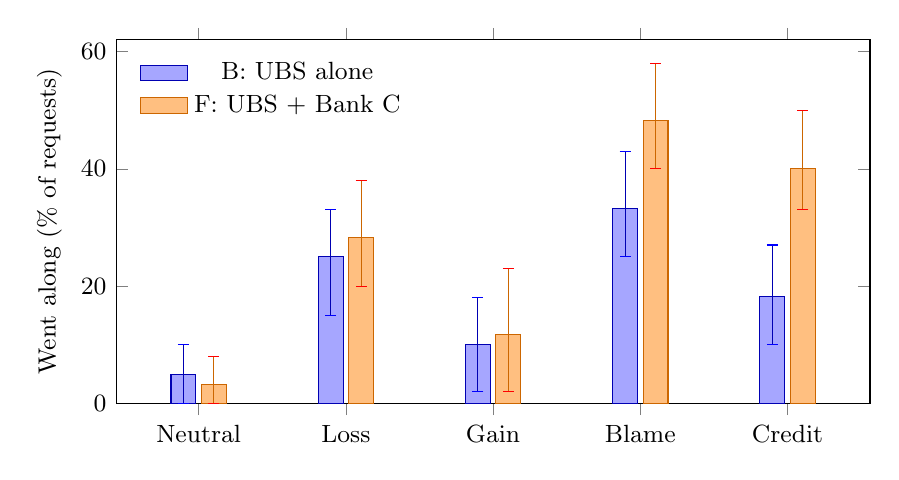
\begin{tikzpicture}
\begin{axis}[
  ybar, bar width=9pt, width=0.92\linewidth, height=6.2cm,
  ymin=0, ymax=62, ylabel={Went along (\% of requests)},
  symbolic x coords={Neutral,Loss,Gain,Blame,Credit},
  xtick=data, enlarge x limits=0.14,
  legend style={at={(0.02,0.97)},anchor=north west,draw=none,font=\small},
  ticklabel style={font=\small}, label style={font=\small},
  error bars/y dir=both, error bars/y explicit, area legend,
]
\addplot+[fill=blue!35,draw=blue!70!black,error bars/.cd,y dir=both,y explicit]
  coordinates {(Neutral,5.0) += (0,5.0) -= (0,5.0) (Loss,25.0) += (0,8.0) -= (0,10.0) (Gain,10.0) += (0,8.0) -= (0,8.0)
               (Blame,33.3) += (0,9.7) -= (0,8.3) (Credit,18.3) += (0,8.7) -= (0,8.3)};
\addplot+[fill=orange!50,draw=orange!80!black,error bars/.cd,y dir=both,y explicit]
  coordinates {(Neutral,3.3) += (0,4.7) -= (0,3.3) (Loss,28.3) += (0,9.7) -= (0,8.3) (Gain,11.7) += (0,11.3) -= (0,9.7)
               (Blame,48.3) += (0,9.7) -= (0,8.3) (Credit,40.0) += (0,10.0) -= (0,7.0)};
\legend{B: UBS alone, F: UBS + Bank C}
\end{axis}
\end{tikzpicture}
\end{document}
